\begin{frame}
    \frametitle{另一种渲染器:点云渲染器}
    \begin{figure}[H]
        \centering
        \includegraphics[width=1\linewidth,keepaspectratio]{fig_splatting.png}
        \caption{溅射splatting示意图}
        \label{fig:tile_render}
    \end{figure}
    \begin{quote}
        一个空间中的3D Gaussian经过这个过程会形式化地转变为一个相机平面上的2D Gaussian,可以用相机平面位置 $(x_k,y_k)$和2D协方差矩阵$V_c$表示 
    \end{quote}
\end{frame}

\begin{frame}
    \frametitle{Gaussian Splatting \cite{kerbl3DGaussianSplatting2023}}
    高斯“抛雪球”本质上是构建了一个以3D高斯为基本单元的可微点云渲染器,
    将空间中的光度粒子看做若干3D高斯分布,
    每一个高斯分布都可以用如下参数描述
    \begin{enumerate}
        \item 高斯分布均值位置 $\bf{p}$,是一个空间中的三维坐标
        \item 高斯分布的$3\times 3$协方差矩阵$V$,可以理解为一个旋转变换R和一个拉伸变换S的组合 $V=R^TS^TSR$,
            可以简单理解为把一个标准的球形沿着任意三个正交方向的拉伸变形之后得到的椭球
        \item 服从该高斯分布的特征$\bf{X}$,包括颜色和透明度 
    \end{enumerate}
\end{frame}


\begin{frame}
    \frametitle{相机模型:FlipY}
    \begin{figure}[H]
    \centering
    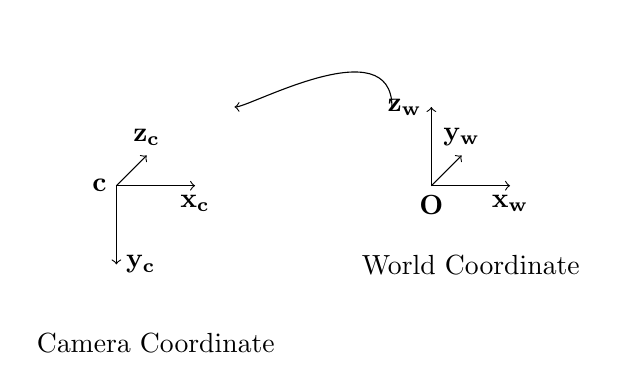
\begin{tikzpicture}[->]
        \begin{scope}[xshift=3.5cm]
            \draw (0,0,0) -- (xyz cs:x=1)node[below]{$\bf{x}_w$};
            \draw (0,0,0) -- (xyz cs:y=1)node[left]{$\bf{z}_w$};
            \draw (0,0,0) -- (xyz cs:z=-1)node[above]{$\bf{y}_w$};
            \node (O) at (0,0,0) [below] {$\bf{O}$};
        \end{scope}
        \draw[->] (3,1) .. controls +(up:1cm) and +(right:0.2cm) .. (1, 1);
        \begin{scope}[xshift=-0.5cm]
            \draw (0,0,0) -- (xyz cs:x=1)node[below]{$\bf{x}_c$};
            \draw (0,0,0) -- (xyz cs:y=-1)node[right]{$\bf{y}_c$};
            \draw (0,0,0) -- (xyz cs:z=-1)node[above]{$\bf{z}_c$};
            \node (P) at (0,0,0) [left] {$\bf{c}$};
        \end{scope}
        \node (A) at (0, -2) {Camera Coordinate};
        \node (B) at (4, -1) {World Coordinate};
    \end{tikzpicture}
    \caption{FlipY Camera Model}
    \label{fig:flip_y_camera}
\end{figure}
\end{frame}

\begin{frame}
    \frametitle{相机模型}
    如图\ref{fig:flip_y_camera}所示,一个正常的右手系世界坐标系$\bf{x_w,y_w,z_w}$和原点$\bf{O}$下,
    相机视角的局部坐标系$\bf{x_c,y_c,z_c}$和相机原点在世界坐标系下的坐标 $\bf{c}$
    $$\left[\begin{matrix} 
        \vec{x}_c \\ \vec{y}_c \\ \vec{z}_c 
    \end{matrix}\right]=
    \left[\begin{matrix} 
        x_{c0} & x_{c1} & x_{c2} \\ 
        y_{c0} & y_{c1} & y_{c2} \\ 
        z_{c0} & z_{c1} & z_{c2} 
    \end{matrix}\right]
    \left[\begin{matrix} 
        \vec{x} \\ \vec{y} \\ \vec{z} 
    \end{matrix}\right]=
    R\left[\begin{matrix} 
        \vec{x} \\ \vec{y} \\ \vec{z} 
    \end{matrix}\right]$$
\end{frame}

\begin{frame}
    \frametitle{视角变换}

    在相机确定之后,任意一个世界坐标$(p_{wx},p_{wy},p_{wz})$都可以经过一个旋转
    和一个平移变换到相机坐标系$(p_{cx},p_{cy},p_{cz})$之中,我们不妨引入齐次坐标的概念
    
    来确定一个$4\times 4$的变换矩阵$\bf{M}$,使得
    
    $[p_{cx},p_{cy},p_{cz},1]=[p_{wx},p_{wy},p_{wz},1]\bf{M}$
    
    并且可以推导出$\bf{M}$的表达式
    
    $$[p_{wx},p_{wy},p_{wz},1]
    \left[\begin{matrix} 
        x_{c0} & y_{c0} & z_{c0} & 0 \\ 
        x_{c1} & y_{c1} & z_{c1} & 0 \\ 
        x_{c2} & y_{c2} & z_{c2} & 0 \\ 
        -\vec{c}\cdot\vec{x}_c &-\vec{c}\cdot\vec{y}_c &-\vec{c}\cdot\vec{z}_c & 1 
    \end{matrix}\right]=[p_{cx},p_{cy},p_{cz}, 1]$$
    
    这里的M被称为View Matrix视角矩阵。
\end{frame}


\begin{frame}
    \frametitle{经过变换的高斯}
    $g_V(x)=\frac{1}{2\pi \sqrt{|V|}}e^{-\frac{1}{2}x^TV^{-1}x}$
    \begin{itemize}
        \item $V$是一个$3\times 3$的协方差矩阵, $|V|$是它的行列式
        \item $x$是一个$3\times 1$的列向量
        \item 高斯变换的好处在于,其傅里叶变换依然是高斯形式:$g_V(x)\leftrightarrow G_V(\omega)=e^{-\frac{1}{2}\omega^TV\omega}=2\pi \sqrt{|V|}g_{V^{-1}}$
    \end{itemize}
    将变换视作重参数化 $y = Mx$
    $g_V(M^{-1}y)=\frac{1}{2\pi\sqrt{|V|}}e^{-\frac{1}{2}(M^{-1}y)^TV^{-1}M^{-1}y}=\frac{|M|}{2\pi\sqrt{|MVM^T|}}e^{-\frac{1}{2}y^T(MVM^T)^{-1}y}=|M|g_{MVM^T}(y)$
    \begin{quote}
    则经过变换得到的y依然服从正态分布,此正态分布是可以定量计算的
    两个高斯分布的卷积也很方便计算: $g_V(x)\otimes g_W(x)=g_{V+W}(x)$
    \end{quote}
\end{frame}

\begin{frame}
    \frametitle{空间往相机平面投影}
    \begin{columns}[c]
        \begin{column}{0.58\textwidth} % Left column width
            \begin{figure}[H]
                \centering
                \includegraphics[width=1\linewidth,keepaspectratio]{fig_surface_splatting.png}
                \caption{可微的高斯变换}
                \label{fig:diff_gaussian_splatting}
            \end{figure}
        \end{column}
        \begin{column}{0.4\textwidth} % Right column width
            $\Phi(t)=[\bold{u}_i,\bold{v}_i,\bold{p}_i]\left[\begin{matrix} \bold{t} \\ 1 \end{matrix}\right]$

            $\bold{x}=m_i(\bold{t})=\left[\begin{matrix} \frac{u_xt_u+v_xt_v+p_x}{u_zt_u+v_zt_v+p_z} \\  \frac{u_yt_u+v_yt_v+p_y}{u_zt_u+v_zt_v+p_z} \end{matrix}\right]$
        \end{column}
    \end{columns}
    \begin{quote}
        从而可以计算Jacobian 
        $$J_i=\left[\begin{matrix}\frac{\partial x}{\partial t_u} & \frac{\partial x}{\partial t_v} \\ \frac{\partial y}{\partial t_u} & \frac{\partial y}{\partial t_v} \end{matrix}\right]=\frac{1}{p_z^2}\left[\begin{matrix}u_xp_z-p_xu_z & v_xp_z - p_xv_z\\ u_yp_z-p_yu_z & v_yp_z-p_yv_z \end{matrix}\right]$$
    \end{quote}
\end{frame}

\begin{frame}
    \frametitle{分块光栅化}
    \begin{figure}[H]
        \centering
        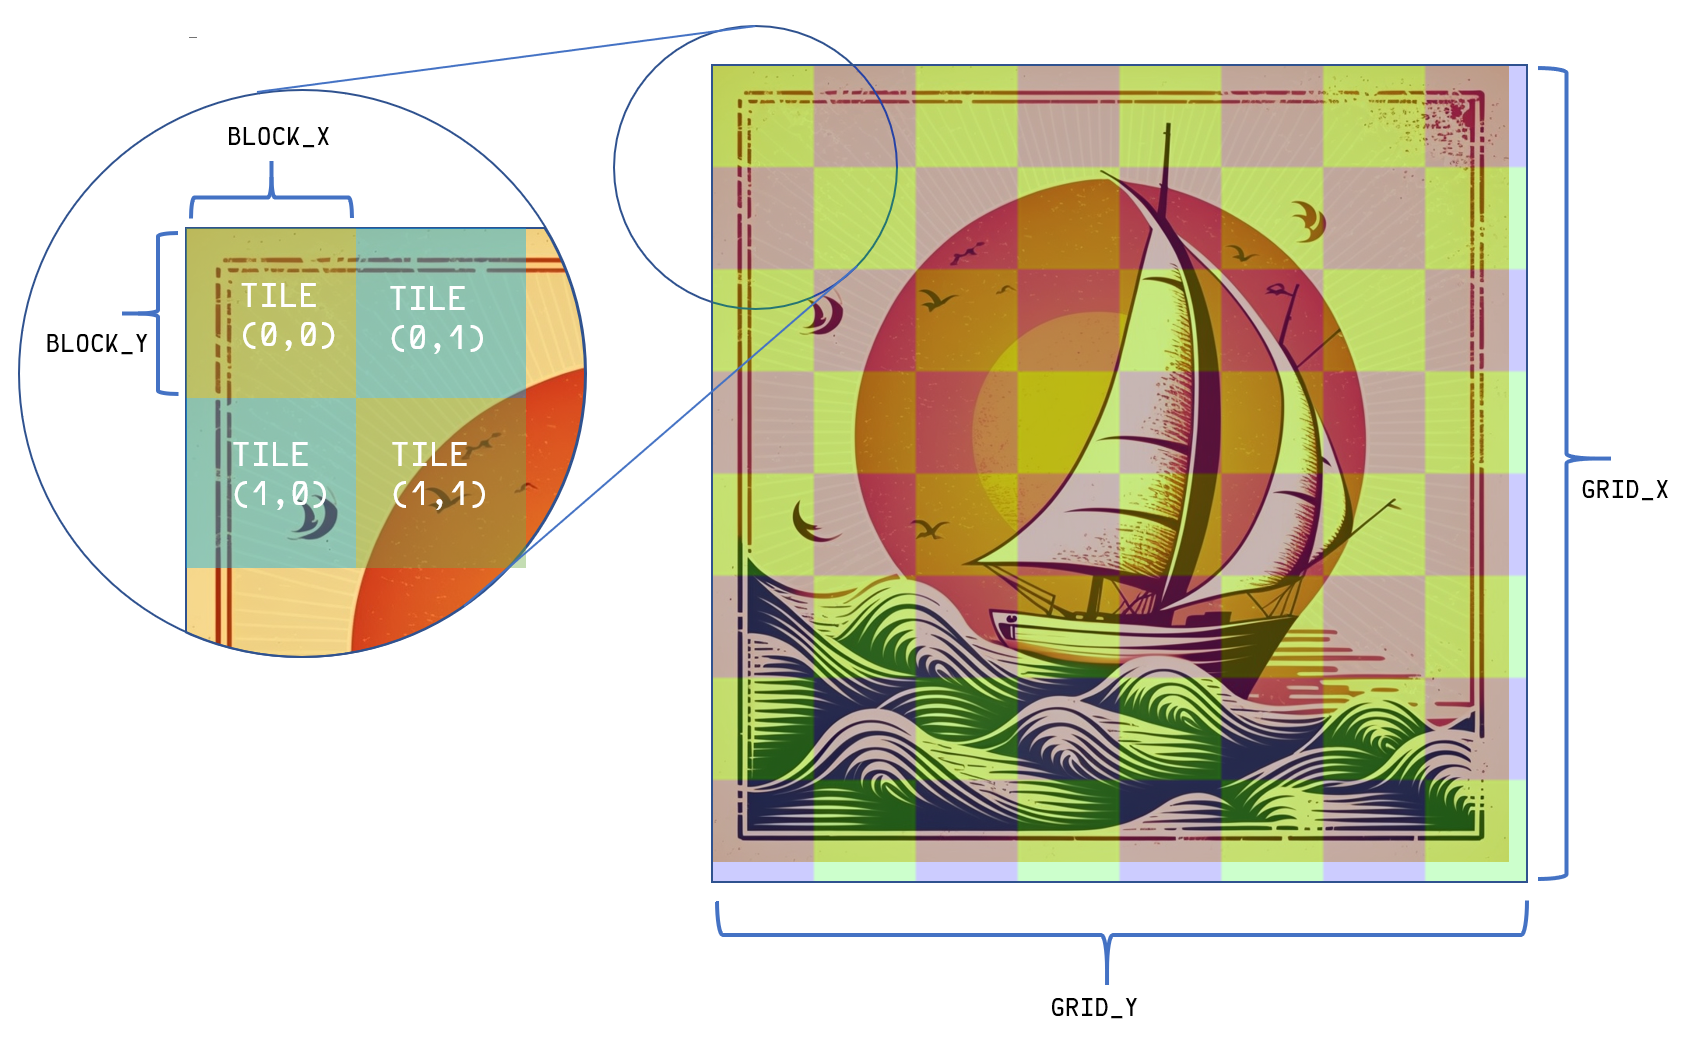
\includegraphics[width=1\linewidth,keepaspectratio]{fig_tile_based_raster.png}
        \caption{分块光栅化}
        \label{fig:tile_render}
    \end{figure}
\end{frame}

\begin{frame}
    \frametitle{分片光栅化}
    \begin{enumerate}
        \item 计算相机的视角变换矩阵和仿射变换矩阵的Jacobian
        \item 将空间转化为为相机局部坐标(变换$\bf{p}$,不变V)
        \item 将相机表面为若干小块(tile),每个小块负责渲染$16\times 16$个像素
        \item 对于每一个tile,可以得到会投影到这个tile上的高斯分布,并将他们按照z轴大小排序
        \item 在NDC中向着相机平面投影,将3D高斯转换为相机平面上的2D高斯分布
        \item 进行band-limit处理来防止aliasing 
        \item 并依排序顺序进行$\alpha$混合,最终得到图像
    \end{enumerate}
\end{frame}

\begin{frame}
    \frametitle{块内$\alpha$混合}
    \begin{quote}
        在经过上述过程之后,每一个块都得到了一个从近到远对应的图像空间Gaussian序列,
        之后我们希望将这个Gaussian列按照一定的透明度顺序进行叠合。需要指出,基于点的高斯
        $\alpha$混合与之前NeRF中的体渲染混合是等价的。
    \end{quote}
    In NeRF
    $C=\sum\limits_{i=1}\limits^{N} T_i(1-exp(-\sigma_i\delta_i))\mathbf{c}_i$, where $T_i=exp(-\sum\limits_{j=1}\limits^{i-1} \sigma_j\delta_j)$
    合并之后,可以把颜色写成每个点颜色的加权和
    $C=\sum\limits_{i}\limits^{N} T_i\alpha_i\mathbf{c}_i$
    此处
    $\alpha_i = (1-exp(-\sigma_i\delta_i))$, $T_i=\prod\limits_{j=1}\limits^{i-1}(1-\alpha_i)$
\end{frame}

\begin{frame}
    \frametitle{后续工作}
    \begin{quote}
        虽然距离Gaussian Splatting源码正式放出不到三个月,arxiv上已经有了一些工作
    \end{quote}
    \begin{itemize}
        \item Dynamic 3D Gaussian \cite{luitenDynamic3DGaussians2023} 来自原作者团队,将Gaussian Splatting 扩展到动态
        \item Dream Gausssian \cite{tangDreamGaussianGenerativeGaussian2023} 将DreamFusion\cite{pooleDreamFusionTextto3DUsing2022}中的NeRF部分替换为3D Gaussian,从而实现了更好的生成质量
    \end{itemize}
\end{frame}